\documentclass[tikz,border=2pt]{standalone}
\usepackage{tikz}
\begin{document}
  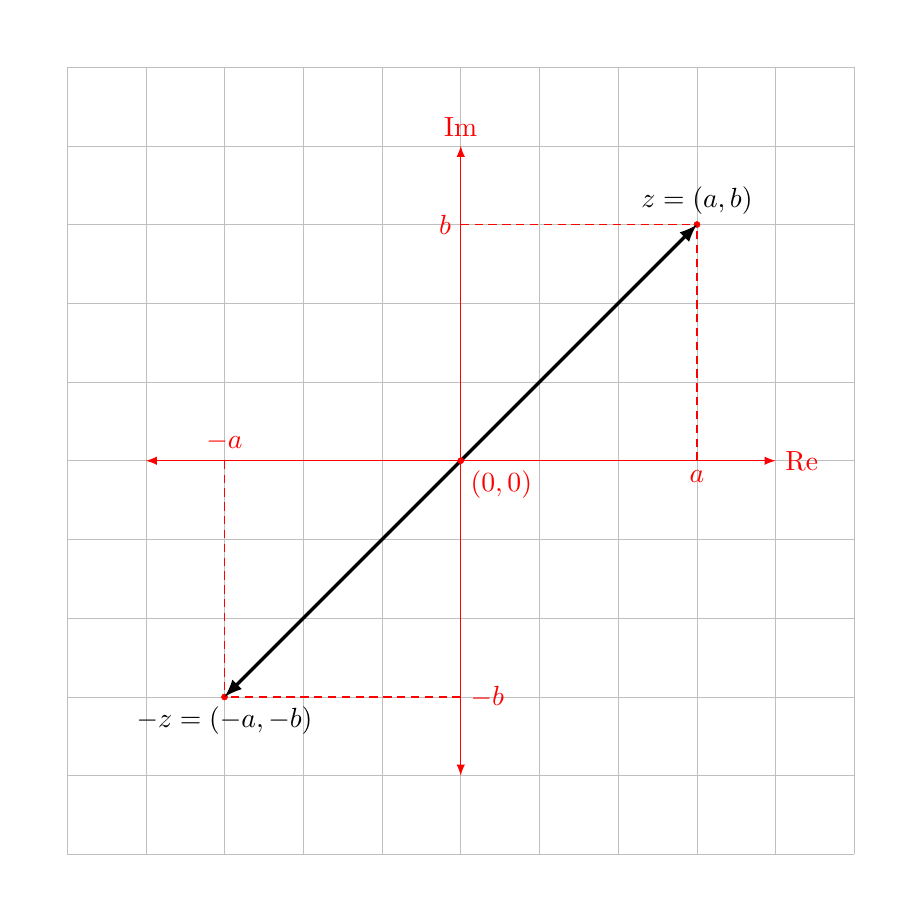
\begin{tikzpicture}
    \fill[white] (-5.5,-5.5) rectangle (5.5,5.5);
    \draw[lightgray,very thin] (-5,-5) grid (5,5);
    \draw (0,0) node[red,below right]{$(0,0)$};
    \draw[red,latex-latex] (-4,0) -- (4,0) node[right]{Re};
    \draw[red,latex-latex] (0,-4) -- (0,4) node[above]{Im};
    \draw[red,densely dashed] (3,0) -- (3,3);
    \draw[red,densely dashed] (0,3) -- (3,3);
    \draw[red,densely dashed] (-3,0) -- (-3,-3);
    \draw[red,densely dashed] (0,-3) -- (-3,-3);
    \draw[red] (3,0) node[below]{$a$};
    \draw[red] (-3,0) node[above]{$-a$};
    \draw[red] (0,3) node[left]{$b$};
    \draw[red] (0,-3) node[right]{$-b$};
    \filldraw[red] (3,3) circle(1pt) node[black,above]{$z=(a,b)$};
    \filldraw[red] (-3,-3) circle(1pt) node[black,below]{$-z=(-a,-b)$};
    \draw[very thick,-latex] (0,0) -- (3,3);
    \draw[very thick,-latex] (0,0) -- (-3,-3);
    \filldraw[red] (0,0) circle(1pt);
  \end{tikzpicture}
\end{document}

